\documentclass[a4paper,12pt]{article}

\usepackage[utf8]{inputenc}
\usepackage[italian]{babel}
\usepackage{amsmath}
\usepackage{geometry}
\usepackage{listings}
\usepackage{hyperref}
\usepackage{graphicx}
\usepackage{booktabs}
\usepackage{caption}
\usepackage{subcaption}
\usepackage{float}

\geometry{margin=2.5cm}

\graphicspath{{../}}

\lstset{
    basicstyle=\ttfamily\small,
    breaklines=true,
    frame=single,
    numbers=left,
    numberstyle=\tiny,
    xleftmargin=1.5em
}

\title{Relazione Laboratorio HPC -- Esercitazione 2\\
\large Timing, Matrix Multiplication, Network e Storage}
\author{Federico Becchi}
\date{Giugno 2026}

\begin{document}

\maketitle
\tableofcontents
\newpage

% =========================================================
\section{Ambienti di calcolo}

I test sono stati eseguiti su due ambienti distinti:

\begin{itemize}
    \item \textbf{PC locale}: MacBook Air con chip Apple M3, macOS 26.3.1, architettura ARM64
    \item \textbf{Cluster HPC Ateneo}: nodo \texttt{ui01.hpc.unipr.it}, Intel Xeon Gold 6238R @ 2.20 GHz, architettura x86\_64 con supporto AVX512, gestito tramite SLURM
\end{itemize}

% =========================================================
\section{Timing}

\subsection{Descrizione del programma}

Il programma \texttt{timing.c} misura due tipologie di tempo distinte tramite la funzione \texttt{clock\_gettime}:

\begin{itemize}
    \item \textbf{REALTIME} (\texttt{CLOCK\_REALTIME}): il tempo di parete (\textit{wall-clock time}), ossia il tempo reale trascorso dall'inizio alla fine del programma.
    \item \textbf{CPUTIME} (\texttt{CLOCK\_PROCESS\_CPUTIME\_ID}): il tempo effettivo di utilizzo della CPU da parte del processo.
\end{itemize}

Il programma esegue due operazioni sequenziali: una \texttt{sleep(1)} (che blocca il processo senza consumare CPU) e un ciclo di 500 milioni di iterazioni floating point. Si aspetta quindi che:
\[
\text{REALTIME} \approx 1\,\text{s (sleep)} + t_{\text{loop}} > \text{CPUTIME} \approx t_{\text{loop}}
\]

\subsection{Script di esecuzione}

\subsubsection{PC -- \texttt{timing.sh}}
\begin{lstlisting}[language=bash]
#!/bin/sh
gcc timing.c -o timing -O2
./timing > timing_pc.csv
\end{lstlisting}

\subsubsection{Cluster -- \texttt{timing.slurm}}
\begin{lstlisting}[language=bash]
#!/bin/sh
#SBATCH --partition=cpu_guest
#SBATCH --qos=cpu_guest
#SBATCH --nodes=1
#SBATCH --cpus-per-task=1
#SBATCH --time=0-00:05:00

gcc -O2 timing.c -o timing
./timing > timing.csv
\end{lstlisting}

\subsection{Risultati}

\begin{table}[H]
\centering
\begin{tabular}{lcc}
\toprule
\textbf{Ambiente} & \textbf{REALTIME (s)} & \textbf{CPUTIME (s)} \\
\midrule
PC (MacBook Air M3)        & 1.3803 & 0.3752 \\
Cluster (Xeon Gold 6238R)  & 1.9682 & 0.9680 \\
\bottomrule
\end{tabular}
\caption{Risultati del test di timing su PC e Cluster.}
\end{table}

\subsection{Considerazioni}

In entrambi gli ambienti si osserva che REALTIME $>$ CPUTIME, confermando il comportamento atteso: il secondo trascorso in \texttt{sleep(1)} incrementa solo il wall-clock time, non il tempo CPU.

Il CPUTIME sul PC (0.3752 s) \`e inferiore rispetto al cluster (0.9680 s): il chip Apple M3 con architettura ARM64 e frequenza boost pi\`u alta esegue il ciclo floating point in modo pi\`u efficiente. Il REALTIME del cluster \`e pi\`u alto perch\'e include, oltre all'\texttt{sleep}, un loop pi\`u lento.

\begin{figure}[H]
\centering
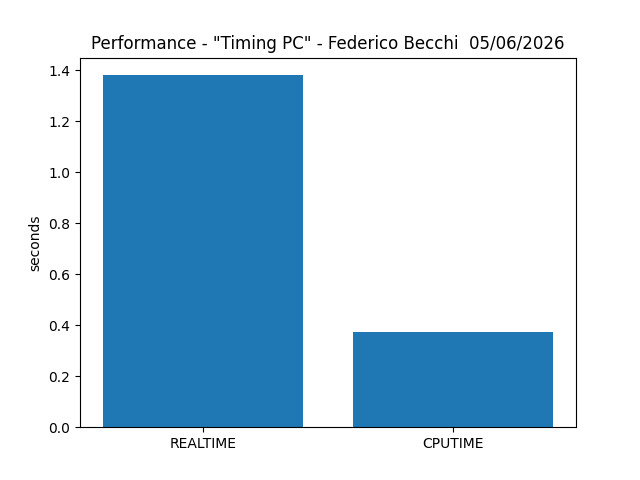
\includegraphics[width=0.75\textwidth]{timing/timing.png}
\caption{Grafico comparativo REALTIME vs CPUTIME su PC e Cluster.}
\end{figure}

% =========================================================
\section{Matrix Multiplication}

\subsection{Descrizione}

L'esercizio esplora le prestazioni della moltiplicazione matriciale $C = A \times B$ con matrici quadrate di dimensione $N=1024$ in singola precisione floating point (\texttt{float}). Vengono confrontate diverse ottimizzazioni:

\begin{itemize}
    \item Implementazione seriale con \textbf{GCC/ICC} (cicli annidati)
    \item Ottimizzazione tramite libreria \textbf{GSL} (\texttt{gsl\_blas\_sgemm})
    \item Parallelizzazione \textbf{OpenMP}
    \item Accelerazione \textbf{GPU} (CUDA)
\end{itemize}

La metrica di prestazione usata \`e \textbf{GFLOP/s}, calcolata come:
\[
\text{GFLOP/s} = \frac{N^3 \times 2}{10^9 \times \text{tempo(s)}}
\]
Per $N=1024$: GFLOP $\approx 2.15$.

\subsection{CPU -- Versione seriale e GSL}

\subsubsection{PC -- \texttt{mm.sh}}

Per compilare su macOS \`e stato necessario installare la libreria GSL tramite Homebrew:
\begin{lstlisting}[language=bash]
brew install gsl
\end{lstlisting}
e adattare i path nella compilazione:
\begin{lstlisting}[language=bash]
gcc $OPT -o mm mm.c \
    -I/opt/homebrew/opt/gsl/include \
    -L/opt/homebrew/opt/gsl/lib \
    -lgsl -lgslcblas
\end{lstlisting}

Lo script esegue il programma due volte: una senza GSL (cicli naive) e una con l'opzione \texttt{-g} (routine BLAS ottimizzata).

\subsubsection{Cluster -- \texttt{omp\_mm\_scaling.slurm}}

Sul cluster \`e disponibile anche il compilatore Intel (\texttt{icc}) che sfrutta le istruzioni AVX/AVX512 del processore Xeon. I test includono combinazioni di compilatori (gcc/icc), ottimizzazioni vettoriali (AVX) e GSL.

\subsection{Risultati CPU}

\begin{table}[H]
\centering
\begin{tabular}{llcc}
\toprule
\textbf{Ambiente} & \textbf{Configurazione} & \textbf{Tempo (s)} & \textbf{GFLOP/s} \\
\midrule
PC       & gcc (seriale)      & 0.65 & 3.31  \\
PC       & gcc + GSL          & 0.30 & 7.09  \\
\midrule
Cluster  & gcc (seriale)      & 1.42 & 1.52  \\
Cluster  & gcc + GSL          & 0.10 & 22.13 \\
Cluster  & icc (seriale)      & 1.42 & 1.52  \\
Cluster  & icc + GSL          & 0.10 & 22.10 \\
Cluster  & icc + AVX          & 0.18 & 12.20 \\
Cluster  & icc + AVX + GSL    & 0.10 & 22.19 \\
\bottomrule
\end{tabular}
\caption{Prestazioni moltiplicazione matriciale CPU, $N=1024$, singola precisione.}
\end{table}

\subsection{OpenMP -- scaling}

\subsubsection{Script \texttt{omp\_mm\_scaling.slurm}}

\begin{lstlisting}[language=bash]
#SBATCH --cpus-per-task=32

for N in 1024; do
  for NT in 1 2 4 8; do
    ./omp_mm -n $N -t $NT -c $HOSTNAME-$NT
  done
done > $FILENAME
\end{lstlisting}

Il programma \texttt{omp\_mm.c} parallelizza i cicli di inizializzazione e calcolo tramite la direttiva \texttt{\#pragma omp parallel for}.

\subsubsection{Risultati OpenMP}

\begin{table}[H]
\centering
\begin{tabular}{llccc}
\toprule
\textbf{Ambiente} & \textbf{Thread} & \textbf{Tempo (s)} & \textbf{GFLOP/s} & \textbf{Speedup} \\
\midrule
PC      & 1 & 0.94 & 2.27  & 1.00 \\
PC      & 2 & 0.47 & 4.53  & 2.00 \\
PC      & 4 & 0.26 & 8.29  & 3.62 \\
PC      & 8 & 0.16 & 13.49 & 5.88 \\
\midrule
Cluster & 1 & 1.43 & 1.50  & 1.00 \\
Cluster & 2 & 0.72 & 2.99  & 1.99 \\
Cluster & 4 & 0.36 & 5.89  & 3.97 \\
Cluster & 8 & 0.34 & 6.35  & 4.21 \\
\bottomrule
\end{tabular}
\caption{Scaling OpenMP per la moltiplicazione matriciale, $N=1024$.}
\end{table}

\subsection{Grafici CPU}

\begin{figure}[H]
\centering
\begin{subfigure}[b]{0.48\textwidth}
    
\includegraphics[width=\textwidth]{matrixMul/PLOTTING/PC/CPU/matrixMul.png}
    \caption{PC (MacBook Air M3)}
\end{subfigure}
\hfill
\begin{subfigure}[b]{0.48\textwidth}
    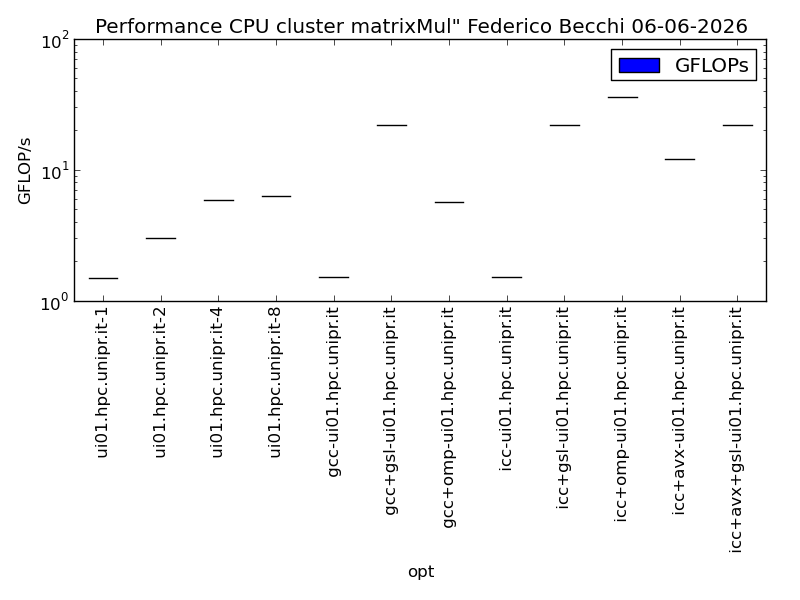
\includegraphics[width=\textwidth]{matrixMul/PLOTTING/Cluster/CPU/matrixMul.png}
    \caption{Cluster (Xeon Gold 6238R)}
\end{subfigure}
\caption{Prestazioni CPU (GFLOP/s) con diverse ottimizzazioni, $N=1024$.}
\end{figure}

\subsection{Considerazioni CPU}

\begin{itemize}
    \item La versione seriale naive \`e pi\`u lenta sul cluster rispetto al PC, probabilmente per via della frequenza di clock pi\`u alta del chip M3 e della migliore cache locality.
    \item L'uso di GSL porta un enorme vantaggio su entrambi gli ambienti: sul cluster si passa da 1.52 a 22.13 GFLOP/s (+1357\%), perch\'e GSL invoca routine BLAS altamente ottimizzate con vettorizzazione AVX.
    \item Lo speedup OpenMP sul PC \`e quasi lineare fino a 4 thread; a 8 thread si riduce (5.88x invece di 8x ideale) per contention sulla memoria condivisa.
    \item Sul cluster a 8 thread lo speedup si ferma a 4.21x: il nodo assegnato nella partizione \texttt{cpu\_guest} ha limitazioni sulle risorse fisiche disponibili.
\end{itemize}

% =========================================================
\subsection{GPU -- CUDA}

\subsubsection{Descrizione}

Il programma \texttt{matrixMul} \`e il sample CUDA di NVIDIA che esegue la moltiplicazione matriciale su GPU tramite kernel CUDA ottimizzato con tiling (\textit{shared memory}). Le matrici $A$ ($1024 \times 1024$) e $B$ ($1024 \times 1024$) vengono caricate in memoria GPU e il risultato $C$ viene calcolato in parallelo dai thread CUDA.

\subsubsection{Script \texttt{matrixMul.slurm}}

\begin{lstlisting}[language=bash]
#SBATCH --partition=gpu
#SBATCH --gres=gpu:p100:1

module load cuda

WA=1024; HA=1024; WB=1024; HB=1024
./matrixMul -wA=$WA -hA=$HA -wB=$WB -hB=$HB >> mm_GPU.$HOSTNAME.csv
\end{lstlisting}

\subsubsection{Risultati GPU}

\begin{table}[H]
\centering
\begin{tabular}{llccc}
\toprule
\textbf{Ambiente} & \textbf{Device} & \textbf{Tempo (ms)} & \textbf{GFLOP/s} & \textbf{Risultato} \\
\midrule
Cluster  & NVIDIA Tesla P100 (cc 6.0) & 1.006 & 2135.34 & PASS \\
PC       & --                          & --    & --       & Non disponibile \\
\bottomrule
\end{tabular}
\caption{Prestazioni GPU CUDA, matrici $1024 \times 1024$ singola precisione.}
\end{table}

La GPU non \`e disponibile sul MacBook Air M3, che utilizza l'architettura Metal di Apple (senza supporto CUDA). Il test \`e stato eseguito unicamente sul cluster nella partizione \texttt{gpu} richiedendo una GPU NVIDIA Tesla P100 (architettura Pascal, compute capability 6.0).

\begin{figure}[H]
\centering

\includegraphics[width=0.6\textwidth]{matrixMul/PLOTTING/Cluster/GPU/matrixMul.png}
\caption{Prestazioni GPU CUDA (GFLOP/s), Cluster -- NVIDIA Tesla P100.}
\end{figure}

\subsection{Confronto CPU vs GPU}

\begin{table}[H]
\centering
\begin{tabular}{llc}
\toprule
\textbf{Dispositivo} & \textbf{Configurazione migliore} & \textbf{GFLOP/s} \\
\midrule
PC CPU       & OpenMP 8 thread         &  13.49   \\
Cluster CPU  & icc + AVX + GSL         &  22.19   \\
Cluster GPU  & NVIDIA Tesla P100 CUDA  & 2135.34  \\
\bottomrule
\end{tabular}
\caption{Confronto prestazioni di picco ottenute con $N=1024$.}
\end{table}

La GPU offre un fattore di accelerazione di circa \textbf{96$\times$} rispetto alla migliore configurazione CPU sul cluster, evidenziando il vantaggio dell'architettura SIMT per carichi di lavoro massicciamente paralleli.

% =========================================================
\section{Bandwidth e Latency di Rete}

\subsection{Descrizione}

I benchmark \texttt{mpi\_bandwidth.c} e \texttt{mpi\_latency.c} misurano le prestazioni della rete di interconnessione usando scambi di messaggi MPI punto-a-punto:

\begin{itemize}
    \item \textbf{Bandwidth}: invia messaggi di dimensione crescente (da 8~KB a 163~KB, step 8~KB) tra coppie di task MPI, misurando la banda in MB/s.
    \item \textbf{Latency}: scambia 100 messaggi da 1 byte con ping-pong tra 2 task, calcolando la latenza media in microsecondi.
\end{itemize}

Vengono testati due scenari:
\begin{itemize}
    \item \textbf{Intra-nodo}: entrambi i task sullo stesso nodo (comunicazione via shared memory).
    \item \textbf{Inter-nodo}: un task per nodo (comunicazione via rete fisica OmniPath).
\end{itemize}

\subsection{Script di esecuzione}

\subsubsection{PC -- Docker \texttt{band\_lat.sh}}

Sul MacBook Air \texttt{mpirun} non \`e disponibile nativamente. Il test \`e stato eseguito tramite due container Docker (\texttt{wn1}, \texttt{wn2}) sulla stessa macchina, collegati con una rete bridge. È stato necessario aggiungere gli hostname dei container nel \texttt{docker-compose.yml} per permettere la risoluzione dei nomi tra i due container.

\begin{lstlisting}[language=bash]
mpicc mpi_bandwidth.c -o mpi_bandwidth
mpicc mpi_latency.c  -o mpi_latency
mpirun -npernode 2 -np 2 -host wn1:4       mpi_bandwidth 2> band1-$HOSTNAME.csv
mpirun -npernode 1 -np 2 -host wn1:4,wn2:4 mpi_bandwidth 2> band2-$HOSTNAME.csv
mpirun -npernode 2 -np 2 -host wn1:4       mpi_latency   2> lat1-$HOSTNAME.csv
mpirun -npernode 1 -np 2 -host wn1:4,wn2:4 mpi_latency   2> lat2-$HOSTNAME.csv
\end{lstlisting}

I risultati ottenuti sui container Docker non sono rappresentativi di una rete fisica; il confronto significativo è quello tra intra-nodo e inter-nodo sul cluster HPC.

\subsubsection{Cluster -- \texttt{band\_lat.slurm}}

\begin{lstlisting}[language=bash]
#SBATCH --nodes=2
#SBATCH --ntasks-per-node=2
#SBATCH --constraint=omnipath

module load gnu8 openmpi3

mpicc mpi_bandwidth.c -o mpi_bandwidth
mpicc mpi_latency.c  -o mpi_latency

mpirun -npernode 2 -np 2 mpi_bandwidth 2> band1-$HOSTNAME.csv  # intra-nodo
mpirun -npernode 1 -np 2 mpi_bandwidth 2> band2-$HOSTNAME.csv  # inter-nodo
mpirun -npernode 2 -np 2 mpi_latency   2> lat1-$HOSTNAME.csv   # intra-nodo
mpirun -npernode 1 -np 2 mpi_latency   2> lat2-$HOSTNAME.csv   # inter-nodo
\end{lstlisting}

Il job richiede 2 nodi sulla partizione \texttt{cpu\_guest} con vincolo \texttt{omnipath} (interconnessione Intel OmniPath, 100 Gbps).

\subsection{Risultati -- Bandwidth}

\begin{table}[H]
\centering
\begin{tabular}{lcc}
\toprule
\textbf{Scenario} & \textbf{Banda a 8~KB (MB/s)} & \textbf{Banda a 152~KB (MB/s)} \\
\midrule
Intra-nodo (wn20--wn20) & 1353 & 6015 \\
Inter-nodo (wn20--wn21) & 2123 & 5159 \\
\bottomrule
\end{tabular}
\caption{Bandwidth MPI su cluster (OmniPath), nodo wn20.}
\end{table}

\begin{figure}[H]
\centering
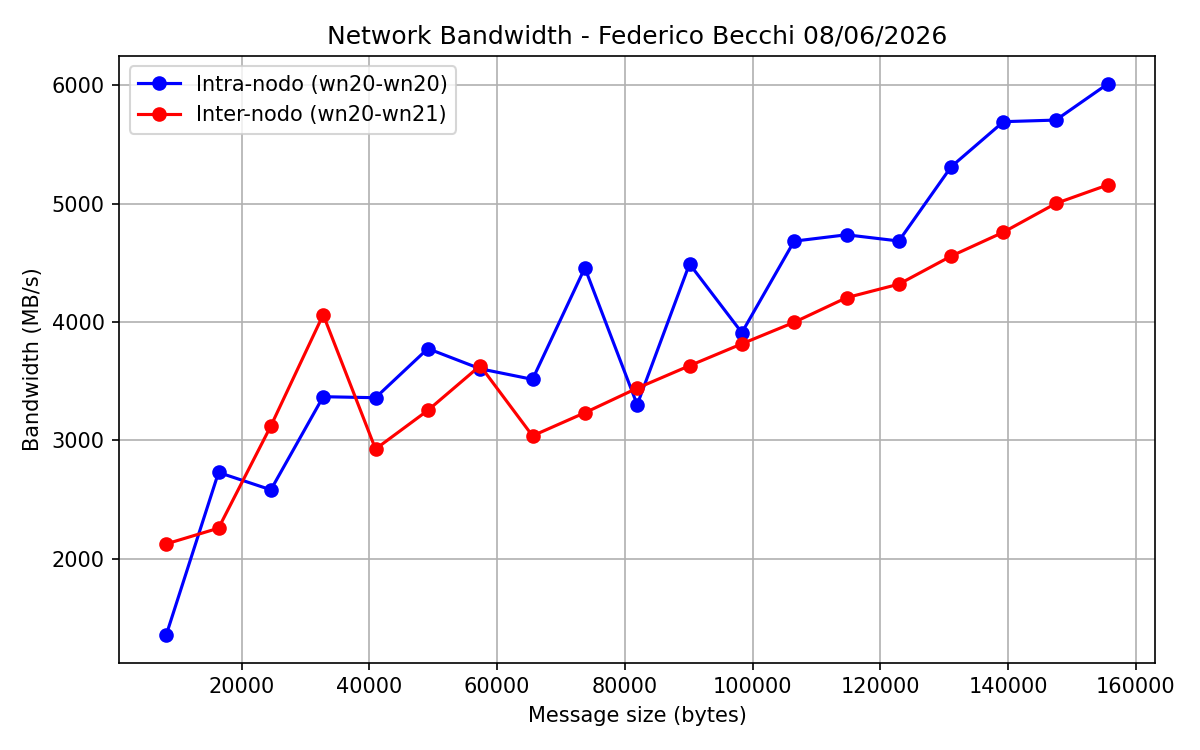
\includegraphics[width=0.75\textwidth]{network/results/Cluster/band.png}
\caption{Bandwidth MPI in funzione della dimensione del messaggio -- Cluster (OmniPath).}
\end{figure}

\subsection{Risultati -- Latency}

\begin{table}[H]
\centering
\begin{tabular}{lcc}
\toprule
\textbf{Scenario} & \textbf{RTT medio ($\mu$s)} & \textbf{Latenza one-way ($\mu$s)} \\
\midrule
Intra-nodo (wn20--wn20) & 1.42 & 0.71 \\
Inter-nodo (wn20--wn21) & 2.33 & 1.16 \\
\bottomrule
\end{tabular}
\caption{Latenza MPI (messaggi da 1~byte, 100 ping-pong), nodo wn20.}
\end{table}

\begin{figure}[H]
\centering
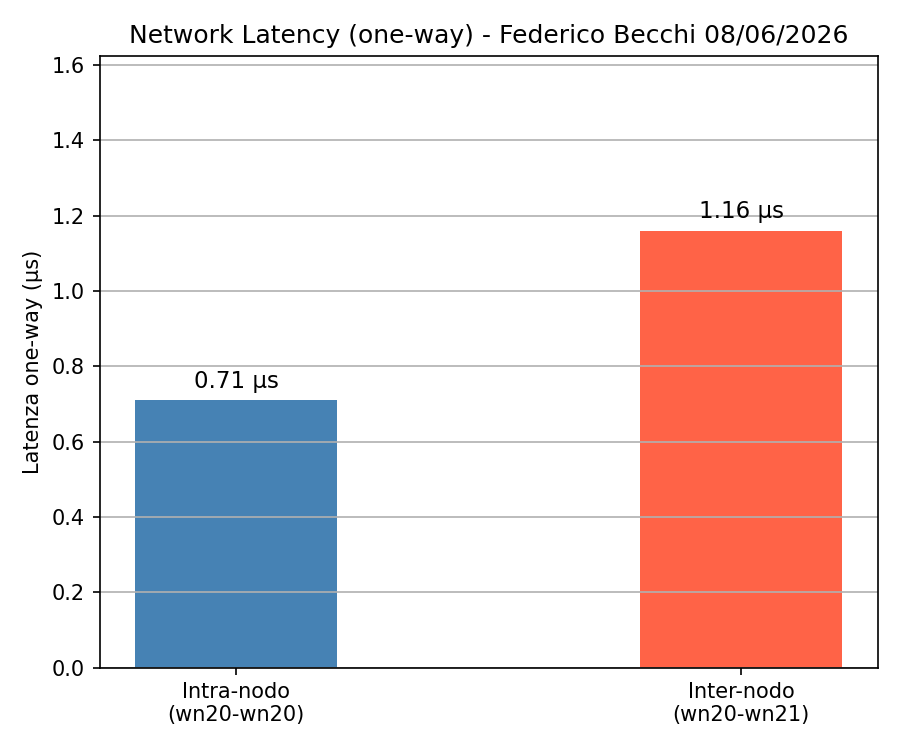
\includegraphics[width=0.6\textwidth]{network/results/Cluster/lat.png}
\caption{Latenza one-way MPI -- Cluster (OmniPath).}
\end{figure}

\subsection{Considerazioni}

\begin{itemize}
    \item La \textbf{banda intra-nodo} raggiunge 6015~MB/s ($\approx$6~GB/s) a messaggi grandi, sfruttando la memoria condivisa del nodo.
    \item La \textbf{banda inter-nodo} (rete OmniPath 100~Gbps) arriva a 5159~MB/s, leggermente inferiore a quella intra-nodo per i messaggi pi\`u grandi.
    \item A messaggi piccoli (8~KB) la situazione si inverte: l'inter-nodo misura 2123~MB/s contro i 1353~MB/s intra-nodo, probabilmente per il diverso protocollo usato da Open MPI per la shared memory (overhead di serializzazione per messaggi piccoli).
    \item La \textbf{latenza one-way} intra-nodo \`e 0.71~$\mu$s, quella inter-nodo 1.16~$\mu$s: entrambe nell'ordine del microsecondo, confermando le elevate prestazioni della rete OmniPath del cluster.
\end{itemize}

% =========================================================
\section{Disk Test}

\subsection{Descrizione}

Il test misura le prestazioni di I/O del disco usando il comando \texttt{dd}, che scrive e poi legge un file temporaneo di dimensione configurabile:

\begin{lstlisting}[language=bash]
dd if=/dev/zero of=$tempfile bs=1M count=$count && sync
dd if=$tempfile of=/dev/null bs=1M count=$count
\end{lstlisting}

Il comando \texttt{sync} forza il flush della cache del kernel sul disco prima di misurare il tempo, rendendo la misurazione di scrittura realistica. Sul cluster il test usa \texttt{count=2048} (2~GB); sul PC \texttt{count=512} (512~MB).

\subsection{PC -- \texttt{disktest.sh}}

Lo script \`e stato adattato per macOS: l'opzione \texttt{conv=fdatasync} non \`e supportata dal \texttt{dd} di macOS, quindi \`e stata sostituita con \texttt{\&\& sync} che produce un effetto equivalente (flush del buffer del kernel). Il test scrive e legge un file da 512~MB (count=512).

\begin{table}[H]
\centering
\begin{tabular}{lcc}
\toprule
\textbf{Operazione} & \textbf{Dimensione} & \textbf{Throughput} \\
\midrule
Scrittura & 512~MB & 962~MB/s \\
Lettura   & 512~MB & 3581~MB/s (3.5~GB/s) \\
\bottomrule
\end{tabular}
\caption{Prestazioni I/O disco -- PC (MacBook Air M3, SSD interno).}
\end{table}

\subsection{Cluster -- \texttt{disktest.slurm}}

Sul cluster il test viene eseguito su tre filesystem diversi:

\begin{itemize}
    \item \textbf{\$HOME}: filesystem NFS condiviso tra tutti gli utenti.
    \item \textbf{\$SCRATCH}: filesystem ad alte prestazioni (Lustre/GPFS), ottimizzato per l'I/O parallelo nei job HPC.
    \item \textbf{\$ARCHIVE}: filesystem di archiviazione per grandi volumi di dati a bassa frequenza di accesso.
\end{itemize}

\begin{lstlisting}[language=bash]
#SBATCH --partition=cpu_guest
#SBATCH --nodes=1

echo "# HOME perf"
cd $HOME && sh disktest.sh

echo "# SCRATCH perf"
cd $SCRATCH && sh disktest.sh

echo "# ARCHIVE perf"
cd $ARCHIVE && sh disktest.sh
\end{lstlisting}

\subsection{Risultati}

\begin{table}[H]
\centering
\begin{tabular}{llcc}
\toprule
\textbf{Ambiente} & \textbf{Filesystem} & \textbf{Scrittura} & \textbf{Lettura} \\
\midrule
PC (MacBook Air M3)  & SSD interno & 962~MB/s  & 3.5~GB/s \\
Cluster -- \$HOME    & NFS         & 304~MB/s  & 3.4~GB/s \\
Cluster -- \$SCRATCH & Lustre      & 884~MB/s  & 2.5~GB/s \\
Cluster -- \$ARCHIVE & --          & \multicolumn{2}{c}{non misurato (\$ARCHIVE non definito)} \\
\bottomrule
\end{tabular}
\caption{Prestazioni I/O disco: PC vs filesystem del cluster HPC.}
\end{table}

\subsection{Considerazioni}

\begin{itemize}
    \item La \textbf{scrittura} pi\`u rapida \`e quella del PC (962~MB/s): il SSD NVMe interno non \`e soggetto a contention e non attraversa la rete.
    \item \textbf{\$SCRATCH} (884~MB/s in scrittura) \`e il filesystem pi\`u performante sul cluster, confermando la sua vocazione all'I/O parallelo ad alto throughput.
    \item \textbf{\$HOME} (304~MB/s in scrittura) \`e pi\`u lento perch\'e \`e un filesystem NFS condiviso: l'I/O passa dalla rete e \`e soggetto a contention tra tutti gli utenti del cluster.
    \item La \textbf{lettura} \`e molto rapida su tutti gli ambienti (2.5--3.5~GB/s) grazie alla cache del kernel (\textit{page cache}): dopo la scrittura, i blocchi restano in memoria e la lettura non accede fisicamente al disco.
    \item La gerarchia di scrittura misurata \`e: $\text{SSD locale} > \text{SCRATCH} \gg \text{HOME}$, in linea con le aspettative architetturali.
\end{itemize}

% =========================================================
\section{Conclusioni}

\begin{itemize}
    \item Il test di \textbf{timing} ha confermato la distinzione tra wall-clock time e CPU time: la \texttt{sleep(1)} incrementa solo il REALTIME, non il CPUTIME. Il chip Apple M3 esegue il ciclo floating point pi\`u velocemente del nodo cluster Xeon (CPUTIME 0.37~s vs 0.97~s).
    \item Nella \textbf{moltiplicazione matriciale CPU}, l'uso di routine BLAS ottimizzate (GSL) porta a un aumento di prestazioni di oltre 14$\times$ rispetto all'implementazione naive. Le istruzioni vettoriali AVX del cluster amplificano ulteriormente il vantaggio.
    \item Il parallelismo \textbf{OpenMP} scala quasi linearmente fino a 4 thread; oltre tale soglia emergono colli di bottiglia legati alla memoria condivisa.
    \item La \textbf{GPU} NVIDIA Tesla P100 supera di circa 96$\times$ la migliore CPU, grazie alle migliaia di core CUDA che eseguono le moltiplicazioni massivamente in parallelo (2135~GFLOP/s vs 22~GFLOP/s).
    \item I benchmark di \textbf{rete MPI} sul cluster mostrano una banda di picco di 6015~MB/s intra-nodo e 5159~MB/s inter-nodo (OmniPath), con latenze one-way rispettivamente di 0.71~$\mu$s e 1.16~$\mu$s.
    \item I test di \textbf{I/O disco} confermano la gerarchia attesa: il SSD locale del PC scrive a 962~MB/s; sul cluster, \$SCRATCH (884~MB/s) supera \$HOME (304~MB/s) perch\'e quest'ultimo \`e un NFS condiviso soggetto a contention.
\end{itemize}

\end{document}
